\documentclass[letter,openright,12pt,spanish]{report}

\title{\textbf{Describir los métodos geométricos algebraicos y desacoplo cinemático.}}
\title{\begin{center}
\includegraphics[scale=1.5]{Escudo.png} 
\end{center}Describir las características de la cinemática directa e inversa de manipuladores paralelos}
\author{Fonseca Camarena Jonathan.\\
		Ing. Mecatr\'onica}
\date{29 de octubre de 2019}
\usepackage{amsmath}
\usepackage{graphicx}
\begin{document}




\maketitle

\section{Cinem\'atica Directa}

El problema cinem\'atico directo consiste en determinar cu\'al es la posici\'on y orientaci\'on del extremo final del robot, con respecto a un sistema de coordenadas que se toma como refrencia, conocidos los valores de las posiciones articulares y los par\'ametros geom\'tricos de los elementos del robot. 

\begin{displaymath}
x=\textit{f}(q)
\end{displaymath}

En general, un robot de "n" grados de libertad est\'a formado por "n" eslabones unidos por "n" articulaciones, de forma que cada par articulaci\'on-eslab\'on constituyen un grado de libertad. A cada eslab\'on se le puede asociar un sistema de refrencia solidario a \'el y, utilizando las transofmaciones homog\'eneas, es posible representar las rotaciones y traslaciones relativas entre los distintos eslabones que componen el rbot. La matriz de transformaci\'on homog\'enea que representa la posici\'on y orientaci\'on relativa entre los distintos sistemas asociados a dos eslabones consecutivos del robot se denomina $^{i-1}A_i$. Del mismo modos, la matriz $^0A_k$, resultante del producto de las matrices $^{i-1}A_i$ con i desde 1 hasta k, es la que representa de forma total o parcial la cadena cinem\'atica que forma el robot con respecto al sistema de referencia inercial asociado a la base. Cuando se considera todos los grados de libertad, a la matriz $^0A_n$ se le denomina T, matriz de transformaci\'on que relaciona la posici\'on y orientaci\'on del extremo final del robot respecto del sistema fijo situado en la base del mismo. As\'i, dado un robot de 6 gdl, se tiene que la osici\'on y orientaci\'on del eslab\\on final vendr\'a dado por la matriz T:\\

\begin{displaymath}
T=^0A_1 \cdot ^1A_2 \cdot ^2A_3... ... ^nA_n
\end{displaymath} 

Para describir la relaci\'on que existe entre dos sistemas de referencia asociados a eslabones, se utiliza la representaci\'on Denavit-Hartenberg (D-H). 

\section{Cinematica Inversa}

EL problema cinem\'atico inverso consiste en encontrar los valores que deben adoptar las coordenadas articulares del robot [ $\textit{q=q}_1,\textit{q}_2,...,\textit{q}_n$ ] para que su extremo se posicione y oriente seg\'un una determinada localizaci\'on espacial. Al contrario que el problema cinem\'atico directo, el c\'alculo de la cinam\'atica inversa no es sencilla ya que conssite en la resoluci\'on de una serie de ecuaciones fuertemen dependiente de la configuraci\'on del robot, adem\'as de existir diferentes \textit{n-uplas} [$\textit{q=q}_1,\textit{q}_2,...,\textit{q}_n$ ] que resuelve el problema.
En la actualidad existen procedimientos gen\'ericos susceptibles de ser progrmados para la resoluci\'on de la cinem\'atica inversa y obtener la \textit{n-upla} de valores articulares que posionen y orienten el extremo final. Sin embargo, el principla inconveniente de estos procedimientos es que son m\'etodos num\'ericos iterativos, que no siempre garantizan tener la soluci\'on en el momento adecuado. De esta manera, a la hora de resolver el problema cinem\'atico inverso es mucho m\'as adecuado encontrar una soluci\'on cerrada. Es decir, encontrar una relaci\'on matem\'atica expl\'icita de la forma:

\begin{displaymath}
q_k=f_k(x, y, z, \alpha, \beta, \gamma)
\end{displaymath}

\begin{displaymath}
k=1...n (grados de libertad)
\end{displaymath}

Para poder conseguir esta relaci\'on suele ser habitual emplear geom\'etricos, que consisten en la utilizaci\'on de las relaciones trigonom\'etricas y la resoluci\'on de los tr\'iangulos formados por los elementos y articulaciones del robot. La mayor\'ia de los robots suele tener cadenas cinem\'aticas relativamente sencillas, y los tres primeros grados de libertad (gdl), que posicionan al robot en el espacio, suelen tener una estructura planar. Esta condici\'on facilita la resoluci\'on de la \textit{n-upla}. Adem\'as, los tres \'ultimos grados de libertad suelen usarse para la orientaci\'on de la herramienta, lo cual permite la resoluci\'on desacolada (descoplo cinem\'atico) de la posici\'on del extremo del robot y de la orientaci\'on de la herramienta. Como alternativa para reoslver el mismo problema se puede recurrir a manipular directamente las ecuaiciones correspondientes al problema cinem\'atico directo. Es decir, a partir de la relaci\'on entre la matriz de transformaci\'on y las ecuaciones en funci\'on de las coordenadas articulares $\textit{q=[q}_1,\textit{q}_2,\textit{q}_3,...,\textit{q}_n]$, es posible despejar las n variables articualaciones $q_i$ en funci\'on de las componentes de los vectores \textbf{n}, \textbf{o}, \textbf{a} y \textbf{p}:

\begin{center}
[
$\begin{matrix}
	n & o & a & p\\
	0 & 0 & 0 & 1\\
\end{matrix}$ ] = [$t_ij$($q_i$,...$q_n$)]
\end{center}

Donde los elementos $t_{ij}$ son funciones de las coordenadas articulares ($q_i$,...,$q_n$)$\cdot $ $e^t$.

La matriz de tranfomaci\'on homog\'enea es una matriz 4 x 4 que transforma un vector de posici\'on expresado en coordenadas homog\'enas desde un sistema de coordenado a otro. En general se representa:

\begin{center}
T = [ $\begin{matrix}
	R_{3x3} & P_{3x1}\\
	F_{1x3} & 1x1\\
\end{matrix}$ ] = [$\begin{matrix}
	\textbf{rotaci\'on} & \textbf{traslaci\'on}\\
	\textbf{perspectiva} & \textbf{escaldo}\\
\end{matrix}$
\end{center}

\section{Robots Paralelos}
En robots paralelos, la cinemática inversa consiste en encontrarlas variables de las juntas activas y pasivas en función de las coordenadas del efector final del robot y puede ser utilizada para controlarla posición del efector final. El modelo cinemático de este tipo de robots tiene ecuaciones algebraicas con múltiples soluciones\\
\\
En la cinemática directa de robots paralelos el problema es determinar la posición del efector final en función de las juntas activas. En general, la solución a este problema no es única, de ahí que la cinemática ha sido objeto de una intensa investigación, por ejemplo, el trabajo reportado por Merlet. Raghavan muestra la solución de la cinemática directa de un manipulador paralelo resolviendo en función de un polinomio. Merlet, Tsai y Ángeles mostraron, de igual manera, que el problema de la cinemática directa es reducir las ecuaciones de posición a un polinomio en función de las variables activas. Sin embargo, la solución del polinomio no asegura la correcta evolución de las variables de las juntas activas y no considera a las juntas pasivas, al ejecutar una tarea dada. Por otro lado, no hay algoritmo conocido que permita la fácil determinación de una postura única para la plataforma móvil.\\
Es importante hacer hincapié en el problema del resultado de la cinemática directa por polinomio. El cálculo puede implicar un gran número de operaciones y por lo tanto puede ser muy sensible a errores numéricos de redondeo; por esta razón la comprobación de la validez de las soluciones con la cinemática inversa es normalmente necesaria\\
\\
Un problema para los métodos numéricos rápidos es que incluso el más rápido es todavía lento para su uso en tiempo real, por ejemplo, para fines de control. Entre los trabajos pioneros publicados que han tratado de resolver éste problema se puede citar a Waldron (1966), quien estudió el movimiento instantáneo por teoría de tornillos en cadenas cinemáticas cerradas, asimismo, se han propuesto otros métodos de análisis. La cinemática diferencial de manipuladores paralelos se complica por la existencia de numerosas cadenas cinemáticas cerradas; recientemente, Mohamed, asimismo, Mohamed y Duffy propusieron la aplicación de la teoría de tornillos recíprocos y Sugimoto a su vez, propuso la utilización del álgebra de motor para el análisis del jacobiano de manipuladores paralelos.\\
\\
La solución de la cinemática directa e inversa, utilizando la integración de la cinemática diferencial, es particularmente importante para los manipuladores de cadenas cinemáticas cerradas cuyas soluciones no existen, son difíciles de obtener, o son demasiado complejas para ser tratadas; el trabajo de Campos, A., R. Guenther, and D. Martins, sobre robots redundantes o paralelos, constituye un buen ejemplo de esto.\\
\\
Chung aborda la cinemática de robots manipuladores seriales redundantes planos, utilizando cadenas virtuales y subcadenas virtuales, para resolver el problema de la cinemática inversa. Chung define a un eslabón virtual como un enlace ficticio que conecta a dos articulaciones. Las ventajas son que reduce la carga de cómputo y logra la manipulación a nivel general mediante la obtención óptima de los ángulos. Entre las desventajas que presenta esta estrategia de análisis se puede mencionar que sólo se aplican a robots seriales planos, es complicado utilizar el método en manipuladores paralelos y tampoco se consideran las velocidades lineales y angulares del robot.

\begin{figure}[htp]
\centering
\includegraphics[width=8cm]{1.jpg}
\caption{RV-M1}
\label{Figura 1}
\end{figure}

Toshio describe al brazo virtual como un manipulador que tiene la misma estructura cinemática de un manipulador real. Su teoría se basa en un sistema que denomina distribuido y que es la representación de la cinemática del manipulador.\\
\\
 Así mismo, utiliza la propagación hacia atrás de redes neuronales. Entre las ventajas del método se pueden mencionar varias; cada subsistema puede trabajar totalmente autónomo, el movimiento de la articulación del manipulador redundante se puede calcular de una manera paralela y distribuida y la redundancia cinemática del manipulador puede ser utilizada positivamente usando sub-brazos virtuales. Algunas desventajas del modelo propuesto por Toshio son que sólo se puede utilizar en robots seriales redundantes planos, asimismo, no toma en cuenta las velocidades lineales y angulares del robot.\\
\\
Para el caso de la síntesis de mecanismos paralelos se utilizan y definen cadenas virtuales seriales y cadenas virtuales paralelas, las cuales se desarrollan sobre la base de la teoría de tornillos. En este caso, cada cadena virtual es propuesta por un análisis exhaustivo de sistemas recíprocos de tornillos.\\
\\
Las cadenas virtuales paralelas constituye un tema de investigación que no ha sido resuelto en su totalidad.Una de las ventajas de aplicar la teoría de tornillos es que se obtienen nuevas estructuras de mecanismos paralelos con ayuda de las cadenas virtuales que define el mismo analista. Entre las desventajas se tiene que sólo se aplica para la obtención de nuevas configuraciones de robots paralelos, no se realiza el modelado de la cinemática directa, inversa y no se obtiene la matriz jacobiana.\\
\\
Por otro lado, como parte del tema de cadenas virtuales, se definen también las cadenas virtuales de Assur y sus aplicaciones en la cinemática diferencial de robots paralelos.\\
\\
 Las cadenas virtuales de Assur son útiles para la obtención de información sobre los movimientos relativos o también para imponer restricciones cinemáticas particulares entre dos eslabones de una cadena cinemática. Entre las ventajas que se pueden mencionar están el hecho de que el método utiliza la cinemática diferencial y el mismo eslabón virtual se utiliza para restringir el movimiento. Asimismo, se pueden definir eslabones virtuales en el plano y en el espacio cartesiano. \\
\\Una de las desventajas de este método radica en que aún considerando el eslabón virtual no se obtiene una matriz jacobiana que considere a las juntas pasivas de robot. Al final se llega a una matriz jacobiana similar a la presentada por Gosselin, C. and J. Angeles[21], donde solo se contemplan juntas activas y no se presentan resultados de simulación para validar los resultados.\\


\section{Postura del Robot}

La Fig. 2, muestra el robot en estudio, con sus tres cadenas cinemáticas independientes, accionadas cada una por un actuador. Como cada una de estas cadenas debe estar ligada, por un lado, a la tierra y por el otro, a la plataforma móvil al mismo tiempo, entonces hay tres puntos de anclaje al suelo y tres puntos de unión a la plataforma móvil.\\

\begin{figure}[htp]
\centering
\includegraphics[width=8cm]{2.jpg}
\caption{RV-M1}
\label{Figura 2}
\end{figure}

\begin{figure}[htp]
\centering
\includegraphics[width=8cm]{3.jpg}
\caption{RV-M1}
\label{Figura 3}
\end{figure}

\begin{figure}[htp]
\centering
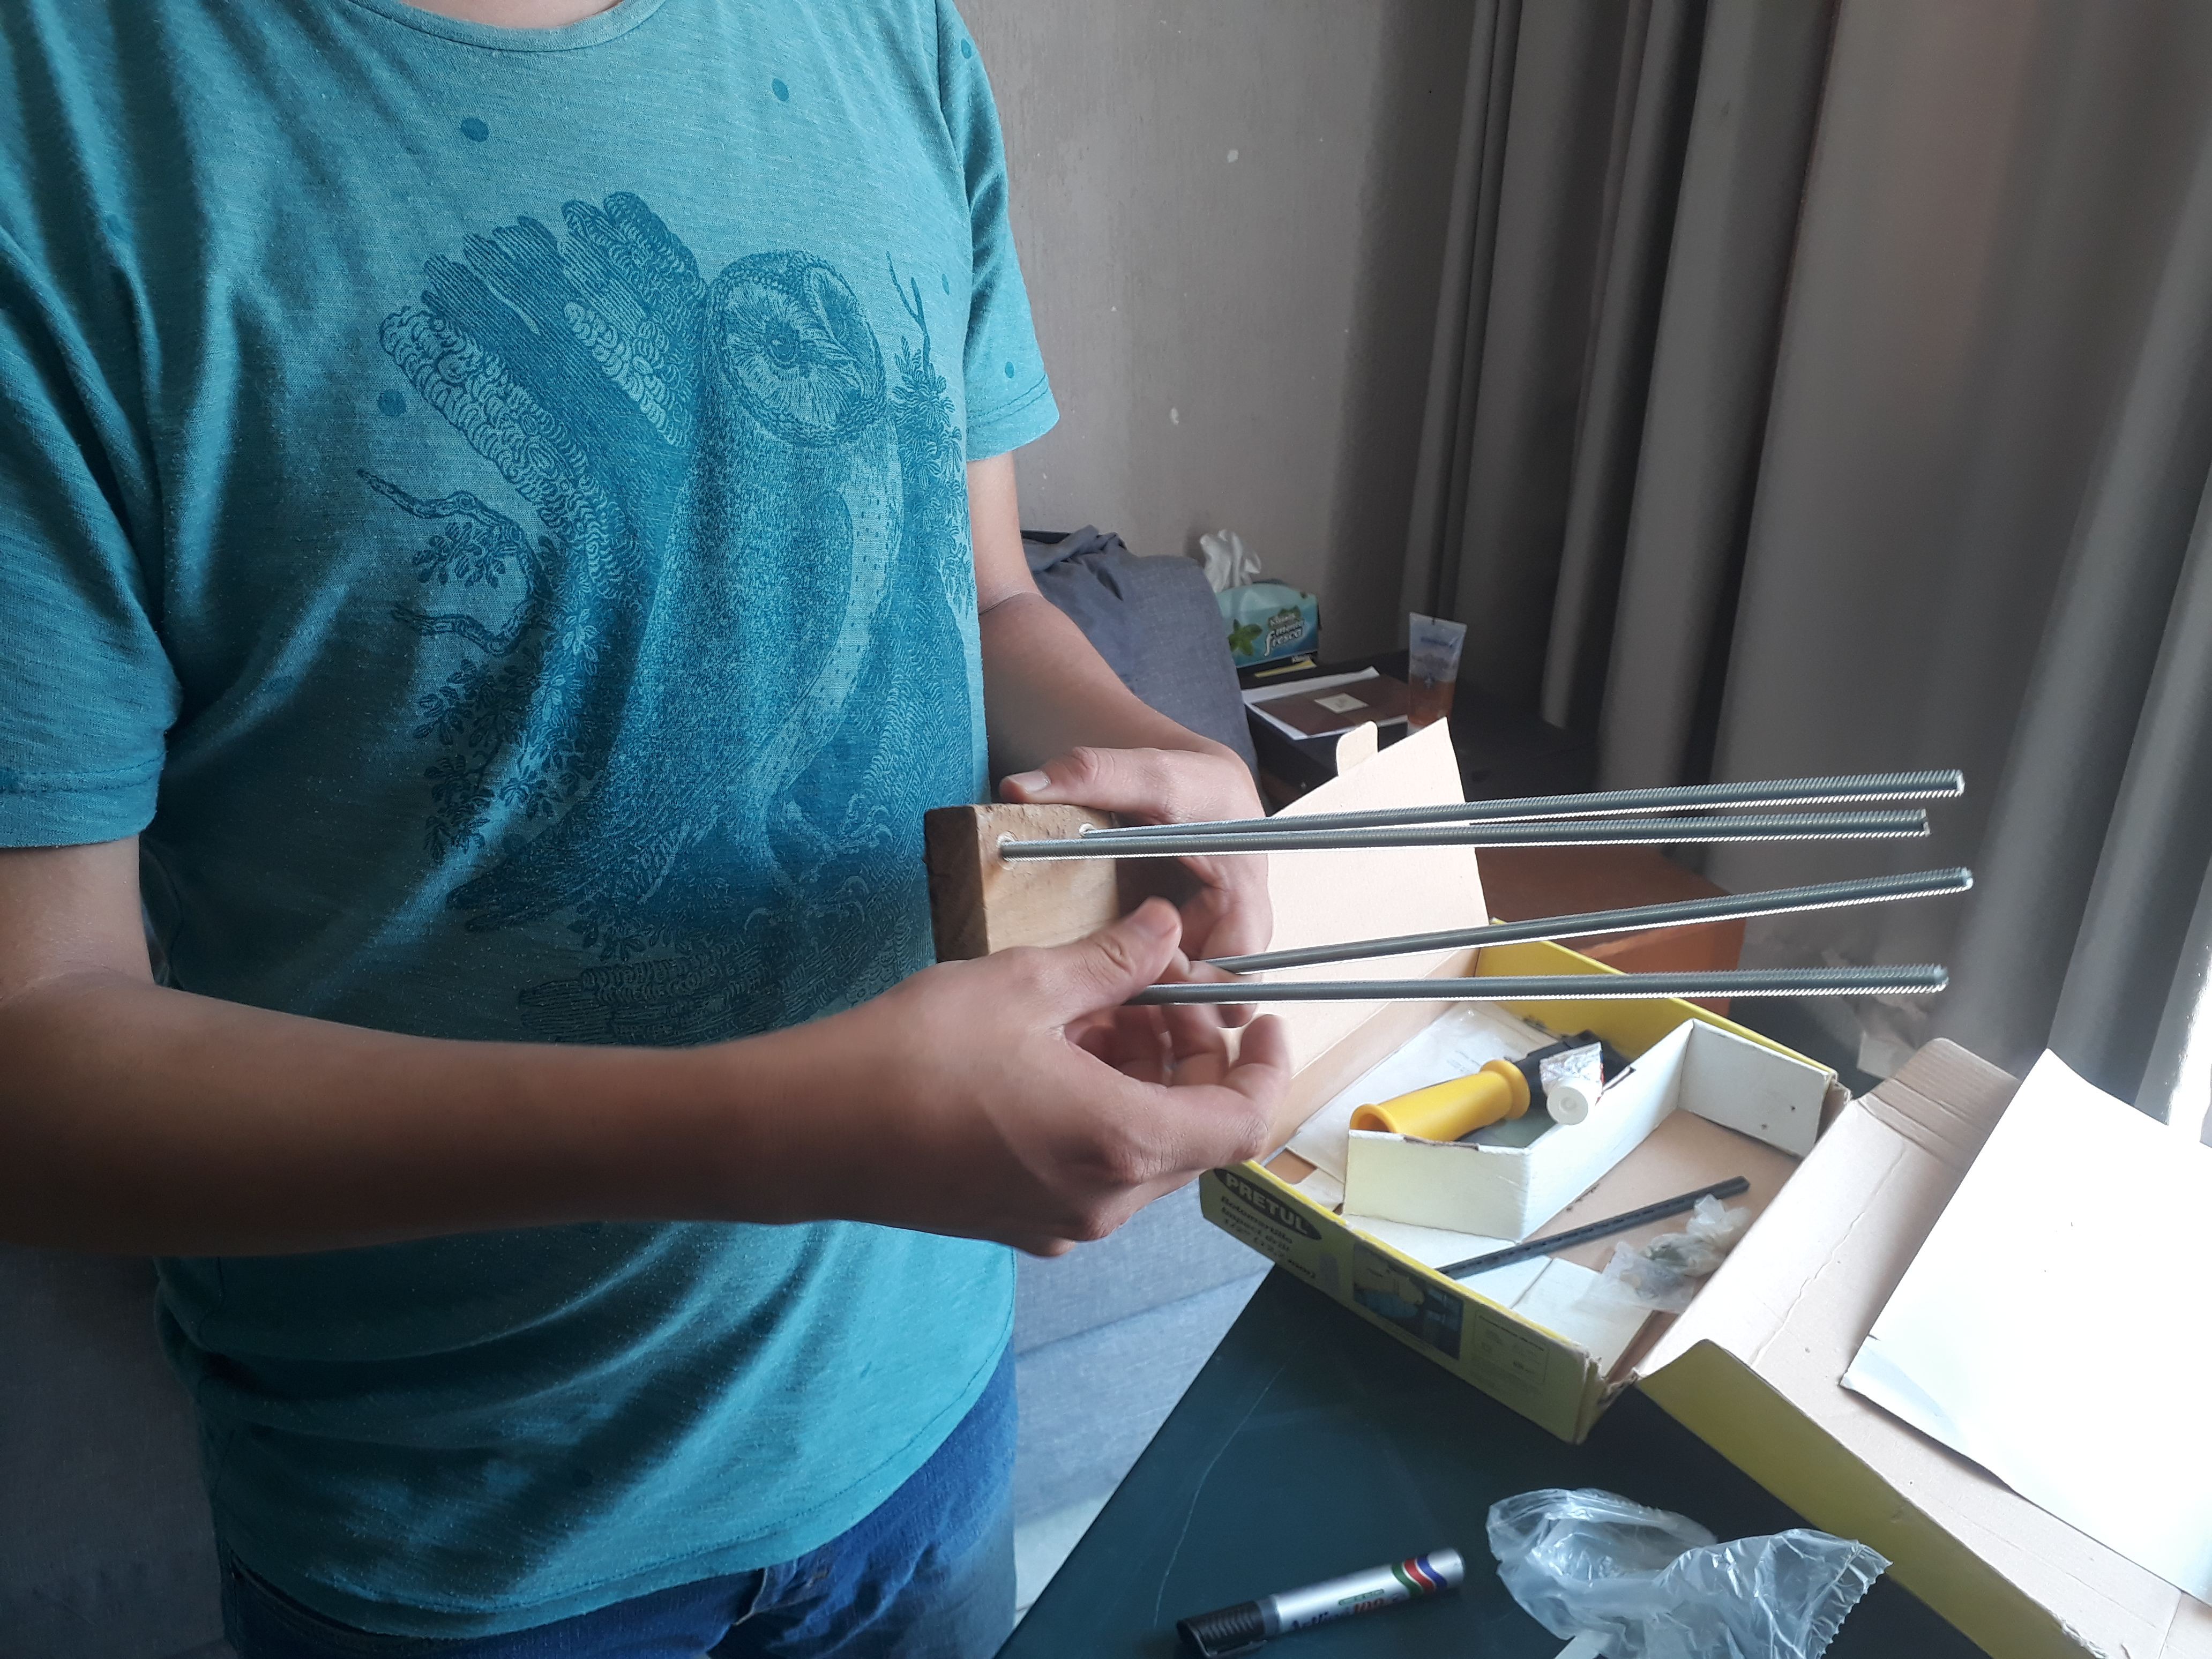
\includegraphics[width=8cm]{4.jpg}
\caption{RV-M1}
\label{Figura 4}
\end{figure}

\begin{figure}[htp]
\centering
\includegraphics[width=8cm]{5.jpg}
\caption{RV-M1}
\label{Figura 5}
\end{figure}

La Figura dos, muestra la postura del robot paralelo plano 3RRR y se puede describir, como sigue:\\
Donde, la coordenada de equiz y Y describe la posición del punto P con respecto al sistema inercial es parcial a cero, es la orientación del manipulador, medida desde el sistema absoluto al sistema local Además, es el vector postura de velocidades del vector. Sea, el vector postura de velocidades del vector, expresado en el sistema local, entonces:



\nocite{*}
\cite{de2017ingenieria}
\bibliographystyle{plain}
\bibliography{biblio}
\end{document}
